\section{Ejercicio 8}
Se decidió separar el diseño en varios bloques que cumplieran tareas específicas, facilitando la implementación.Para comenzar, para evitar problemas de ruido se dividió la implementación en parte digital y analógica.\par
 Los bloques utilizados fueron un generador de rampa con un comparador, un contador para la tasa de refresco y otro contador de pulsos como elemento de medición. Su propuesta de diseño e implementación se presentan a continuación. \par

\subsection{Diseño}

\subsubsection{Generador de Rampa}

Primeramente, se necesitó medir de cierta manera la variación en la tensión provista por el joystick, la cual será proporcional a su posición respecto del eje. Esto se debe a que internamente el joystick cuenta con un pontenciómetro que provee entre $0\,V$ y $5\,V$ de voltaje de salida. Por ende, se diseñó una rampa utilizando un circuito integrado $NE555$, la misma se utilizará para comparar tensiones. \par

\begin{figure}[H]
\centering
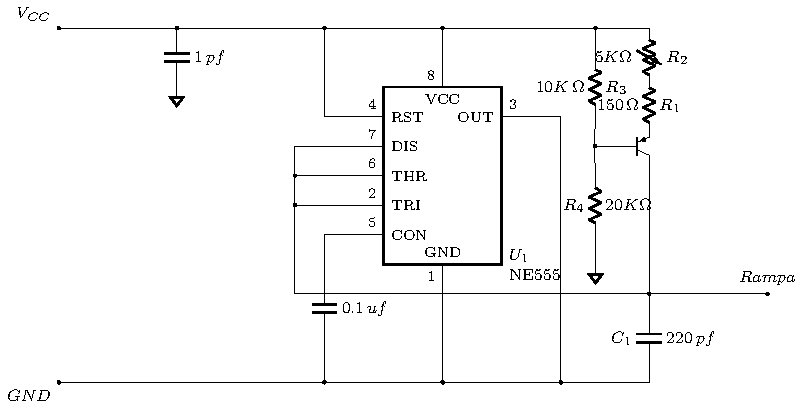
\includegraphics[scale=0.8]{Ejercicio8/Circuitos/Generador_de_rampa.pdf}
\caption{Generador de Rampa con desfasaje}
\label{fig:Generador_de_rampa}
\end{figure}

La rampa representará la carga del capacitor $C_1$ presente en el circuito (\ref{fig:Generador_de_rampa}), dicha carga será constante debido a que el componente anteriormente mencionado está conectado con el colector del transistor PNP que está actuando como fuente de corriente. La tasa de refresco estará dada por la frecuencia de la rampa, siendo la misma constante y de $20\, Hz$. \par
La pendiente $S$ de la rampa estará dada por $S=\frac{I_C}{C_1}=\frac{\Delta V}{\Delta t}$.
Para comenzar, se decidió fijar el valor de $C_1$ en $22\,uf$ tal que sólo sea variable $I_C$. Por otro lado, la corriente en el colector está dada por:

\begin{equation}
I_C=\frac{V_{CC}-V_E}{R_E}
\end{equation}

La tensión en el emisor está determinada por un divisor resistivo dado por:

\begin{equation}
V_E=\frac{R_4}{R_4+R_3} V_{CC} + V_{BE}
\end{equation}

Se fijaron los valores de $R_4$ y $R_3$ en $20K\,\Omega$ y $10K\,\Omega$ respectivamente, tal que la única incógnita sea $R_E$. \par
Se obtuvo un valor nominal para $R_E$ de $2K\,\Omega$. 
Como primer problema a solucionar para el diseño, surgió que rampa provista por el $NE555$ se encontraba entre $5\,V$ y $10\,V$ como se puede ver en la imagen (\ref{fig:Generador_de_rampa_LTSpice}). Esto se debía a la construcción propia del integrado que utiliza comparadores para obtener una señal de salida entre un tercio y dos tercios de la tensión de alimentación ($V_{CC}$), en nuestro caso, $15\,V$.


\begin{figure}[H]
\centering
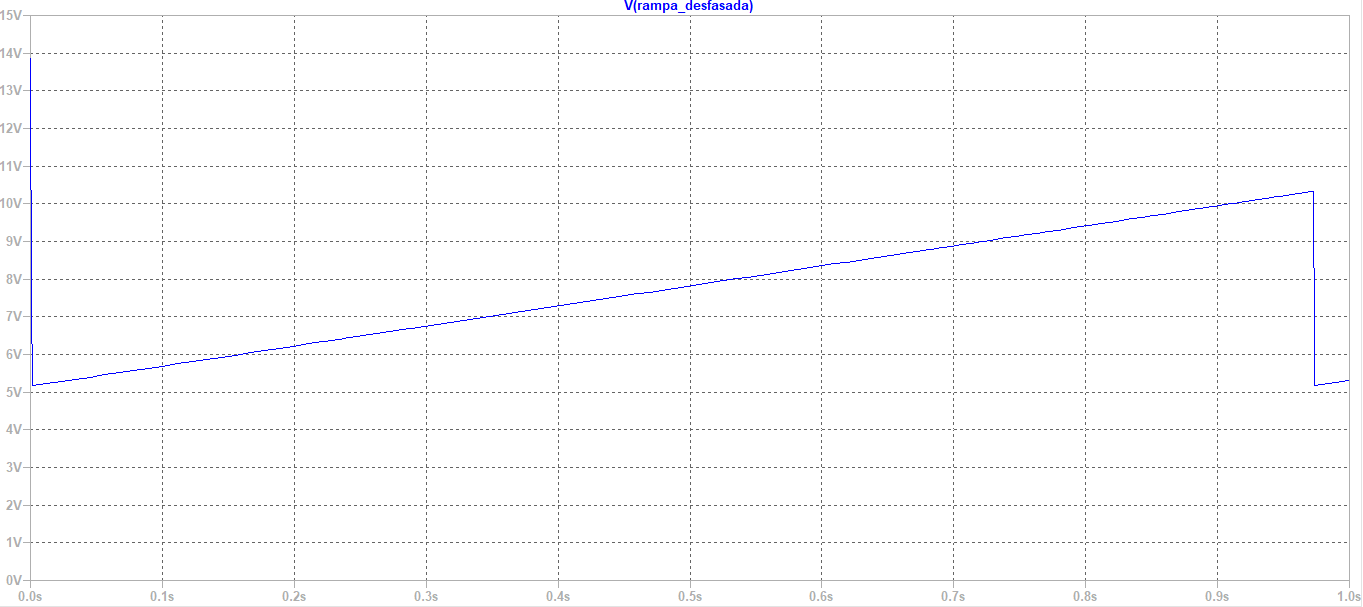
\includegraphics[width=0.7\textwidth]{Ejercicio8/Imagenes/Rampa_desfasada}
\caption{Tensión de la rampa con desfasaje}
\label{fig:Generador_de_rampa_desfasada_LTSpice}
\end{figure}

Por ende, se implementó un amplificador operacional que funcionará como restador para reducir la tensión de salida de la rampa en $5\,V$, utilizando el siguiente circuito:

\begin{figure}[H]
\centering
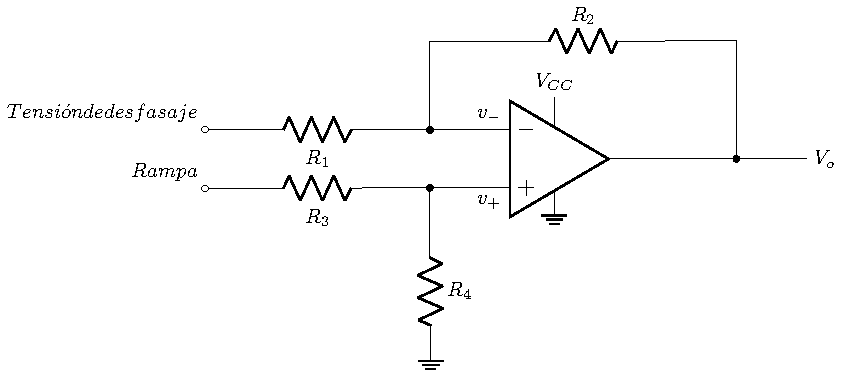
\includegraphics[scale=0.8]{Ejercicio8/Circuitos/Restador.pdf}
\caption{Restador}
\label{fig:Restador}
\end{figure}
\par
La salida del amplificador operacional va a estar dada por:
\begin{equation}
V_o=\frac{-R_2}{R_1}V_2+\left(1+\frac{R_4}{R_3}\right)V_1
\end{equation}
Tomando valores de resistencias equivalentes, obtendremos:
\begin{equation}
V_o=-V_2+V_1
\end{equation}
Siendo $V_1$ la tensión de la rampa y $V_2$ la tensión de desfasaje.\par\par\par
Se obtuvo la siguiente rampa acorde a las necesidades para el trabajo:

\begin{figure}[H]
\centering
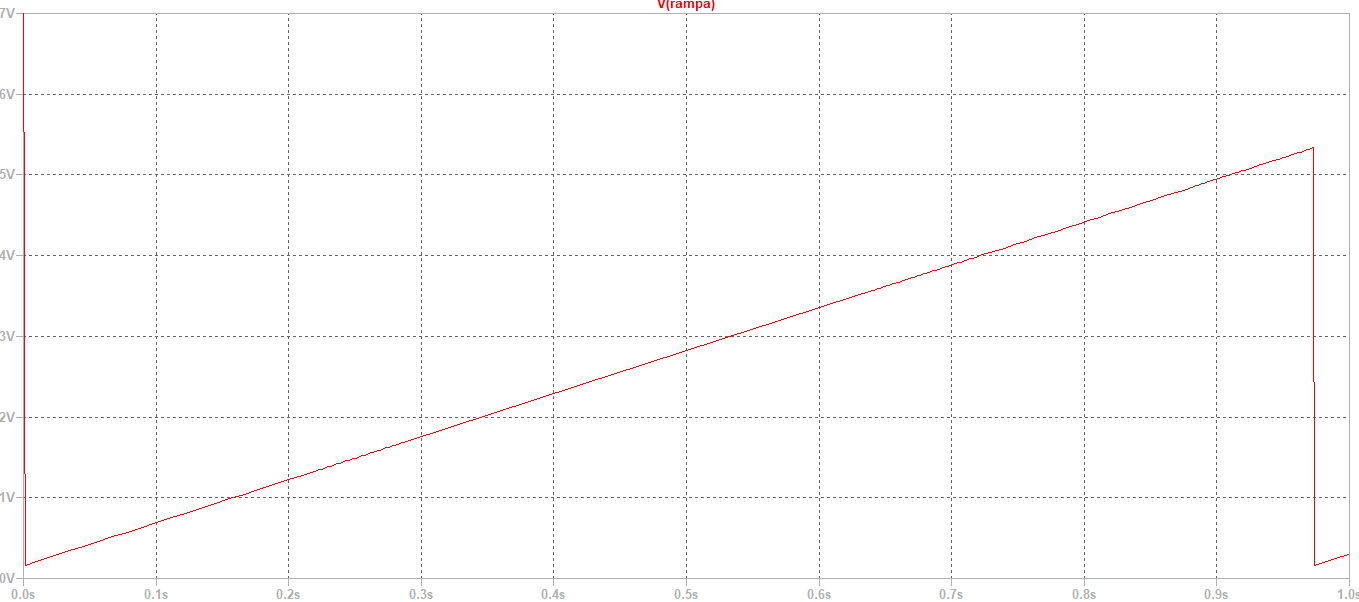
\includegraphics[width=0.7\textwidth]{Ejercicio8/Imagenes/Rampa}
\caption{Tensión de la rampa}
\label{fig:Generador_de_rampa_LTSpice}
\end{figure}



Se considera necesario aclarar la utilización de un buffer entre la salida de la rampa desfasada y el restador para que no se modifiquen los comportamientos entre ambos circuitos.\par


Como segunda decisión de diseño, se implementó un comparador entre la tensión del joystick y la tensión de la rampa. La tensión del joystick variará respecto del tiempo, motivo por el cual se agrega un filtro pasabajo como se puede observar en la figura (\ref{fig:Comparador}) para estabilizar la señal y disminuir el ruido. Como el joystick cuenta con un potenciómetro sólo es necesario agregar un capacitor  a la entrada no inversora del amplificador operacional y tierra, se eligió un capacictor de $1\,uf$.\par
La señal de la rampa estará conectada a la entrada inversora del opamp, mientras que la tensión del joystick estará conectada a la entrada no inversora.

\begin{figure}[H]
\centering
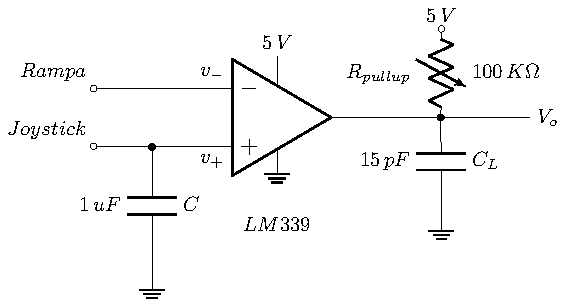
\includegraphics[scale=0.8]{Ejercicio8/Circuitos/Comparador.pdf}
\caption{Comparador de tensiones}
\label{fig:Comparador}
\end{figure}

Cuando la tensión de la rampa sea menor a la tensión del joystick la salida del comparador será de $5\,V$, que representará el 1 lógico del circuito digital. Para el caso contrario, la tensión de salida será de $0\,V$, un 0 lógico para el circuito.

\subsubsection{Tasa de refresco}


\begin{figure}[H]
\centering
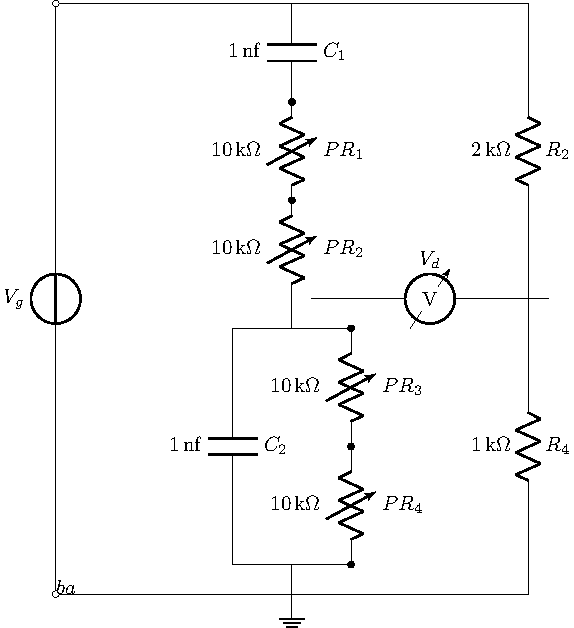
\includegraphics[scale=0.8]{Ejercicio8/Circuitos/Contador&Display.pdf}
\caption{Contador}
\label{fig:Contador&Display}
\end{figure}

\begin{figure}[H]
\centering
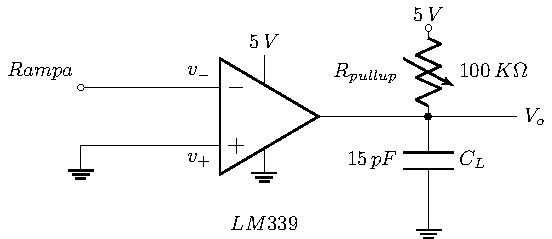
\includegraphics[scale=0.8]{Ejercicio8/Circuitos/Reset.pdf}
\caption{Reset}
\label{fig:Reset}
\end{figure}



\subsubsection{Contador de pulsos}

La frecuencia de clock del contador tendrá que estar relacionada con el período de la rampa. Será indispensable que de ser necesario el contador pueda contar hasta 99 durante un período de la rampa, por lo que deberán entrar 100 pulsos de clock en un período de rampa.  Consecuentemente, como el período de una rampa es constante, la frecuencia del clock del contador de pulsos también lo será, siendo la misma de $2\,KHz$. \par
Para obtener dicho clock se utilizará otro integrado N555 como se puede apreciar en la siguiente figura:

\begin{figure}[H]
\centering
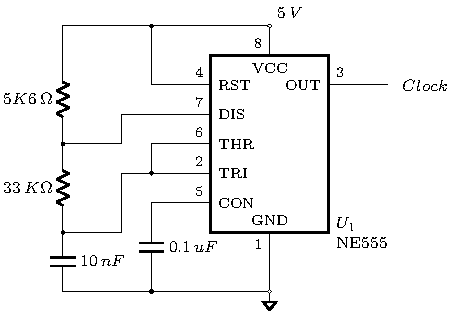
\includegraphics[scale=0.8]{Ejercicio8/Circuitos/Clock.pdf}
\caption{Generador de clock}
\label{fig:Clock}
\end{figure}







\subsection{Conclusiones}